\chapter{La notación asintótica}

\begin{marginfigure}[11\baselineskip]
  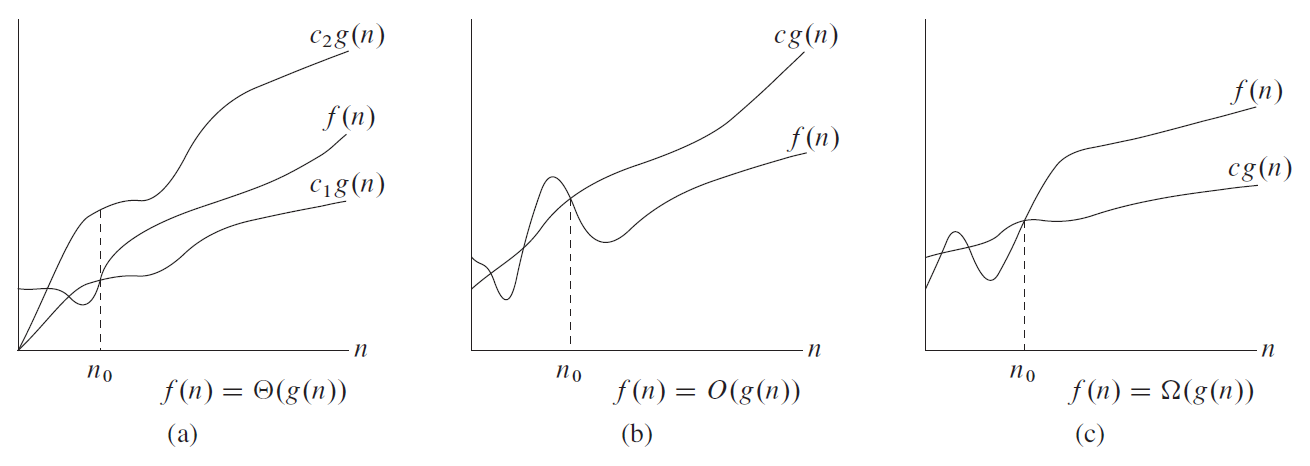
\includegraphics[width=\linewidth]{figuras/big-o}
  \caption{Interpretación gráfica de la notación asintótica. La notación \(f=O(g)\) implica que \(g\) es una cota superior para \(f\).}
\end{marginfigure}

\begin{marginfigure}
  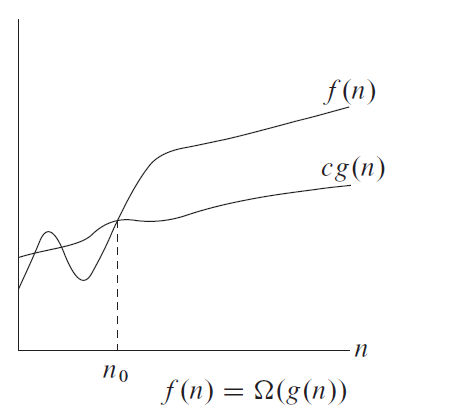
\includegraphics[width=\linewidth]{figuras/big-omega}
  \caption{La notación \(f=\Omega(g)\) implica que \(g\) es una cota inferior para \(f\).}
\end{marginfigure}

\begin{marginfigure}
  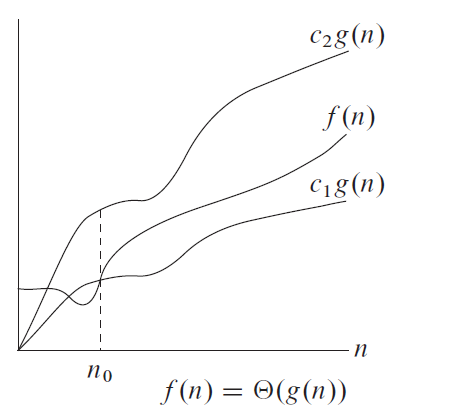
\includegraphics[width=\linewidth]{figuras/big-theta}
  \caption{La notación \(f=\Theta(g)\) implica que \(g\) acota a \(f\) por arriba y por abajo.}
\end{marginfigure}

La \textbf{notación asintótica} es una notación matemática que se utiliza para caracterizar el \emph{orden de crecimiento} de una función; esto es, qué tan rápido crece dicha función suponiendo que la variable independiente incrementa indefinidamente.
La noción básica de esta notación es que, dada una expresión algebraica, los términos de mayor grado crecen más rápido que aquellos de menor grado y, por ende, el efecto que estos últimos tienen sobre el resultado de la función es despreciable cuando la variable es arbitrariamente grande. 
En el análisis de la eficiencia de un algoritmo, la notación asintótica se utiliza para describir el tiempo de ejecución del algoritmo.
La notación asintótica también se utiliza para comparar el desempeño relativo de dos o más algoritmos alternativos para un mismo problema.

\section{Definiciones}

Sea \(n\in\mathbb{N}\) y sean \(f:\mathbb{N}\to\mathbb{R}\) y \(g:\mathbb{N}\to\mathbb{R}\) dos funciones \emph{asintóticamente no-negativas}; esto es, siempre se tiene que \(f(n)\geq 0\) y \(g(n)\geq 0\) a partir de algún valor determinado de \(n\). 

La notación \textbf{O-grande}, que se escribe \(f=O(g)\), indica que \(g\) es una cota superior para \(f\); esto es, \(g\) crece más rápido que \(f\) a partir de cierto valor de \(n\).
Formalmente, \(O(g)\) denota el conjunto de todas aquellas funciones \(f\) para las cuales existen dos constantes, \(c\in\mathbb{R}^+\) y \(n_0\in\mathbb{N}\), tales que \(0\leq f(n)\leq cg(n)\) para toda \(n\geq n_0\). 

La notación \textbf{\(\boldsymbol{\Omega}\)-grande}, que se escribe \(f=\Omega(g)\), indica que \(g\) es una cota inferior para \(f\); esto es, \(f\) crece más rápido que \(g\) a partir de cierto valor de \(n\).
Formalmente, \(\Omega(g)\) denota el conjunto de todas aquellas funciones para las cuales existen dos constantes, \(c\) y \(n_0\), tales que \(0\leq cg(n)\leq f(n)\) para toda \(n\geq n_0\).

La notación \textbf{\(\boldsymbol{\Theta}\)-grande}, que se escribe \(f=\Theta(g)\), indica que \(g\) acota a \(f\) por arriba y por abajo a partir de cierto valor de \(n\).
Formalmente, \(\Theta(g)\) denota el conjunto de todas aquellas funciones para las cuales existen tres constantes, \(c_1,c_2\in\mathbb{R}^+\) y \(n_0\), tales que \(0\leq c_1 g(n)\leq f(n)\leq c_2 g(n)\) para toda \(n\geq n_0\).

\begin{prop}
  Se tiene q. \(f=\Theta(g)\) si y solo si \(f=O(g)\) y \(f=\Omega(g)\).
\end{prop}

La notación \textbf{o-chica}, que se escribe \(f=o(g)\), indica que \(g\) es una cota superior holgada para \(f\).
Esto es, \(o(g)\) denota el conjunto de todas las funciones \(f\) que cumplen que, para toda constante \(c\), existe una constante \(n_0\) tal que \(0\leq f(n)<cg(n)\) para toda \(n\leq n_0\).

La notación \textbf{\(\boldsymbol{\omega}\)-chica}, que se escribe \(f=\omega(g)\), indica que \(g\) es una cota inferior holgada para \(f\).
Esto es, \(\omega(g)\) denota el conjunto de todas las funciones \(f\) que cumplen que, para toda constante \(c\), existe una constante \(n_0\) tal que \(0\leq cg(n)<f(n)\) para toda \(n\geq n_0\).

\begin{prop}
  Si \(f=o(g)\), entonces \(f=O(g)\).
\end{prop}

\begin{prop}
  Si \(f=\omega(g)\), entonces \(f=\Omega(g)\).
\end{prop}

\begin{prop}
  Se tiene que
  \[
    \text{si }\lim_{n\to\infty}\dfrac{f(n)}{g(n)}=\begin{cases}
    0 & \text{entonces }f=o(g)\\
    \infty & \text{entonces }f=\omega(g)\\
    1 & \text{entonces }f=\Theta(g).
    \end{cases}
  \]
\end{prop}

\section{Comparación de funciones por medio de la notación asintótica}

La notación asintótica se puede utilizar para comparar dos funciones y decidir cuál crece más rápido. 
Una forma intuitiva de verlo es trazando las analogías mostradas en la Tabla \ref{tab:func-comp}. 
Esto es posible gracias a que muchas de las propiedades de comparación de los números reales también aplican en la notación asintótica. 
Estas propiedades se describen a continuación, suponiendo que \(f\) y \(g\) son \emph{asintóticamente positivas}.

\begin{table}
  \label{tab:func-comp}
  \caption{Operaciones de comparación de los números reales y su funcionamiento análogo en la notación asintótica.}
  \centering
  \begin{tabular}{cc}
    \toprule 
      Números reales & Notación asintótica\tabularnewline
    \midrule
      \(a\leq b\) & \(f=O(g)\)\tabularnewline
      \(a\ge b\) & \(f=\Omega(g)\)\tabularnewline
      \(a=b\) & \(f=\Theta(g)\)\tabularnewline
      \(a<b\) & \(f=o(g)\)\tabularnewline
      \(a>b\) & \(f=\omega(g)\)\tabularnewline
    \bottomrule
  \end{tabular}
\end{table}

Todos los conjuntos de la notación asintótica poseen la propiedad de \textbf{transitividad}.
Esto es, sea \(h:\mathbb{N}\to\mathbb{R}\) una función asintóticamente positiva, se tiene que:
\begin{itemize}
  \item Si \(f=O(g)\) y \(g=O(h)\), entonces \(f=O(h)\).
  \item Si \(f=\Omega(g)\) y \(g=\Omega(h)\), entonces \(f=\Omega(h)\).
  \item Si \(f=\Theta(g)\) y \(g=\Theta(h)\), entonces \(f=\Theta(h)\).
  \item Si \(f=o(g)\) y \(g=o(h)\), entonces \(f=o(h)\).
  \item Si \(f=\omega(g)\) y \(g=\omega(h)\), entonces \(f=\omega(h)\).
\end{itemize}

Algunos conjuntos de la notación asintótica poseen la propiedad de \textbf{reflexividad}. 
Específicamente: \(f=\Theta(f)\), \(f=O(f)\) y \(f=\Omega(f)\). 
Esto se cumple porque \(f(n)=f(n)\) para toda \(n\).

El conjunto $\Theta$-grande posee la propiedad de \textbf{simetría}.
Así mismo, algunos otros conjuntos poseen la propiedad de \textbf{simetría traspuesta}.
Esto es:
\begin{itemize}
  \item \(f=\Theta(g)\) si y sólo si \(g=\Theta(f)\)
  \item \(f=O(g)\) si y sólo si \(g=\Omega(f)\).
  \item \(f=o(g)\) si y sólo si \(g=\omega(f)\).
\end{itemize}

\marginnote[-4.5\baselineskip]{%
  Cabe mencionar que, dado que $\Theta$-grande posee las propiedades de reflexividad, transitividad y simetría, este conjunto es, de hecho, una \emph{relación de equivalencia}.
}

Por último, la notación asintótica carece de la propiedad de \textbf{tricotomía}, que es la propiedad de los números reales donde, dados dos números $a$ y $b$, siempre se cumple exactamente una de las sig. posibilidades: $a<b$, $a=b$ o $a>b$. 
La notación asintótica carece de esta propiedad porque se puede dar el caso donde no se cumple que \(f=O(g)\) ni que \(f=\Omega(g)\).
Por ejemplo, el comportamiento asintótico de las funciones \(f(n)=n\) y \(g(n)=n^{1+\sin{n}}\) no se puede comparar porque el exponente $1+\sin{n}$ oscila entre 0 y 2, tomando todos los valores intermedios.

\section{Ordenes de crecimiento frecuentes}

A continuación se presentan los órdenes de crecimiento que se observan con mayor frecuencia en las ciencias de la computación, listados de aquél que crece más lento al que crece más rápido.

\begin{enumerate}
  \begin{multicols}{2}
    \item \emph{Constantes}: \(O(1)\)
    \item \emph{Logarítmicos}: \(O(\log n)\)
    \item \emph{Radicales}: \(O(\sqrt{n})\)
    \item \emph{Lineales}: \(O(n)\)
    \item \emph{Súper lineales}: \(O(n\log n)\)
    \item \emph{Cuadráticos}: \(O(n^{2})\)
    \item \emph{Cúbicos}: \(O(n^{3})\)
    \item \emph{Exponenciales}: \(O(2^{n})\)
    \item \emph{Factoriales}: \(O(n!)\)
  \end{multicols}
\end{enumerate}

Se debe tener cuidado sobre cómo interpretar la lista anterior, ya que la notación asintótica puede ocultar constantes muy grandes y dejar una impresión equivocada de la tasa de crecimiento de una función comparada con otra. 
Por ejemplo, supóngase que se tiene \(f(n)=10^{100}n=O(n)\) y \(g(n)=10n\cdot\log n=O(n\log n)\). 
A pesar de que la notación asintótica indica que \(g\) crece más rápido que \(f\), en realidad se trata de lo opuesto, porque la constante \(10^{100}\) supera por mucho la tasa de crecimiento de \(g\).
Como regla general, si la notación asintótica indica que una función crece más rápido que otra, esto debe interpretarse como que es verdad únicamente para valores muy grandes de \(n\).

\section{Operaciones aritméticas con la notación asintótica}

El comportamiento asintótico de la suma de dos funciones está determinada por la función de mayor orden de crecimiento. 
Esto es:
\[
\begin{aligned}
    O(f)+O(g) &= O(\max\{f,g\})\\
    \Omega(f)+\Omega(g) &= \Omega(\max\{f,g\})\\
    \Theta(f)+\Theta(g) &= \Theta(\max\{f,g\})
\end{aligned}
\qquad
\begin{aligned}
    o(f)+o(g) &= o(\max\{f,g\})\\
    \omega(f)+\omega(g) &= \omega(\max\{f,g\})
\end{aligned}
\]

La multiplicación entre una función y una constante no afecta el
comportamiento asintótico de dicha función. 
Esto es:
\[
\begin{aligned}
    O(cf) &= O(f)\\
    \Omega(cf) &= \Omega(f)\\
    \Theta(cf) &= \Theta(f)
\end{aligned}
\qquad
\begin{aligned}
    o(cf) &= o(f)\\
    \omega(cf) &= \omega(f)
\end{aligned}
\]

Cuando dos funciones se multiplican, ambas contribuyen por igual al
comportamiento asintótico de la función resultante. 
Esto es:
\[
\begin{aligned}
    O(f)\cdot O(g) &= O(f\cdot g)\\
    \Omega(f)\cdot\Omega(g) &= \Omega(f\cdot g)\\
    \Theta(f)\cdot\Theta(g) &= \Theta(f\cdot g)
\end{aligned}
\qquad
\begin{aligned}
    o(f)\cdot o(g) &= o(f\cdot g)\\
    \omega(f)\cdot\omega(g) &= \omega(f\cdot g)
\end{aligned}
\]

\marginnote[-2.5\baselineskip]{%
  \textbf{Literatura consultada}: \textcite{cormen_2009}, pp. 28-29, 43-52; \textcite{skiena_2012} pp. 34-41.
}
